\chapter{Numerical Methods and Error Analysis}
\label{ch:numerics}

Ray tracing a black hole is numerically unforgiving in one specific way:
the observables of Chapter~\ref{ch:shadow} live on the \emph{boundary}
between captured and escaping rays, where trajectories diverge
exponentially (the Lyapunov instability of Chapter~\ref{ch:geodesics}),
and the camera sits a thousand gravitational radii from the region where
all the curvature is. This chapter documents the integrator
(\texttt{DormandPrince54::try\_step} in
\texttt{physics/include/sgr\_physics/integrator.hpp}), the constraint
projection that makes boundary metrology tolerance-independent, the
complex-step differentiation behind the generic-metric path, and the
measured convergence evidence for all three
(\texttt{validation/convergence\_tool}).

\section{The Dormand--Prince 5(4) pair}
\label{sec:dp54}

All geodesics are advanced with the explicit embedded Runge--Kutta pair
of \citet{DormandPrince1980} (``DOPRI5''), the workhorse recommended by
\citet{HairerNorsettWanner1993} and \citet{PressNR2007} for smooth
non-stiff systems. One step from $(x, y)$ with size $h$ evaluates seven
stages
\begin{equation}
k_i = f\Bigl(x + c_i h,\ y + h\sum_{j<i} a_{ij}k_j\Bigr),
\qquad i = 1,\dots,7,
\end{equation}
with the Butcher tableau
\begin{equation}
\renewcommand{\arraystretch}{1.35}
\begin{array}{c|cccccc}
0 & & & & & & \\
\frac15 & \frac15 & & & & & \\
\frac{3}{10} & \frac{3}{40} & \frac{9}{40} & & & & \\
\frac45 & \frac{44}{45} & -\frac{56}{15} & \frac{32}{9} & & & \\
\frac89 & \frac{19372}{6561} & -\frac{25360}{2187} & \frac{64448}{6561}
        & -\frac{212}{729} & & \\
1 & \frac{9017}{3168} & -\frac{355}{33} & \frac{46732}{5247}
  & \frac{49}{176} & -\frac{5103}{18656} & \\
1 & \frac{35}{384} & 0 & \frac{500}{1113} & \frac{125}{192}
  & -\frac{2187}{6784} & \frac{11}{84} \\
\hline
 & \frac{35}{384} & 0 & \frac{500}{1113} & \frac{125}{192}
  & -\frac{2187}{6784} & \frac{11}{84}
\end{array}
\label{eq:butcher}
\end{equation}
whose bottom row gives the fifth-order solution $y^{(5)}$ that is
propagated (\emph{local extrapolation}). The seventh stage is evaluated
at $(x+h,\,y^{(5)})$ — the ``first same as last'' stage — and enters only
the error estimate: the difference between the fifth-order weights and
the embedded fourth-order weights defines the coefficients
$e_1,\dots,e_7$ hard-coded in \texttt{try\_step}, so that
\begin{equation}
\delta_i = h\,(e_1 k_{1,i} + e_3 k_{3,i} + e_4 k_{4,i}
 + e_5 k_{5,i} + e_6 k_{6,i} + e_7 k_{7,i})
\end{equation}
estimates the local truncation error of the \emph{fourth}-order
solution, an upper bound on that of the propagated fifth-order one.

\subsection{Error norm and step control}

The implementation controls the root-mean-square of the component-wise
scaled errors,
\begin{equation}
\epsilon = \sqrt{\frac{1}{N}\sum_{i=1}^{N}
\left(\frac{\delta_i}{{\rm atol} + {\rm rtol}\,
\max(|y_i|, |y^{(5)}_i|)}\right)^{\!2}},
\label{eq:errnorm}
\end{equation}
accepting the step when $\epsilon \le 1$ and proposing
\begin{equation}
h_{\rm next} = h \cdot \mathrm{clamp}\bigl(0.9\,
\epsilon^{-1/5},\ 0.2,\ 5\bigr)
\label{eq:controller}
\end{equation}
— the classical proportional (deadbeat) controller with safety factor
$0.9$ and growth limits; the exponent $-1/5$ reflects the fourth-order
error estimate ($\delta \propto h^5$). (The companion journal paper
loosely called this a ``PI'' controller; the implementation carries no
integral memory, and none proved necessary — the acceptance rate on
production rays exceeds 97 per cent.) For null-ray metrology the
tolerances are ${\rm atol} = {\rm rtol} = 10^{-11}$; the mixed absolute
term matters because state components span $10^{-9}$ (momenta near
turning points) to $10^{3}$ ($t$, $r$ on the camera leg).

Fig.~\ref{fig:stepsize} shows the controller at work along a single
boundary-grazing ray: the step collapses by four orders of magnitude as
the photon winds through the strong-curvature region near $r = 3M$, then
relaxes on the long quiet legs — exactly the behaviour that makes an
adaptive method mandatory here (a fixed step fine enough for the photon
sphere would waste $10^4\times$ the work on the approach).

\begin{figure}
\centering
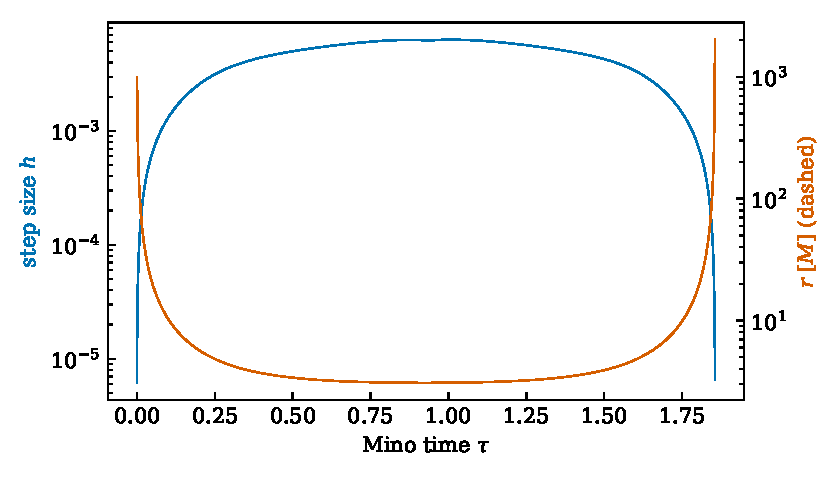
\includegraphics[width=0.8\textwidth]{figures/fig_step_size.pdf}
\caption{Accepted step size $h(\tau)$ (blue, left axis) and radius
$r(\tau)$ (red, right axis) along a ray aimed $0.1\%$ outside the
critical angle (\texttt{convergence\_tool} dump, tolerance $10^{-11}$).
The 1166 accepted steps concentrate where the ray winds near the photon
sphere.}
\label{fig:stepsize}
\end{figure}

\section{Constraint projection}
\label{sec:projection}

The second-order Mino formulation of Chapter~\ref{ch:geodesics} carries
the first integrals $p_r^2 = R(r)$, $p_\theta^2 = \Theta(\theta)$ as
checkable invariants. The decisive design decision of the tracer is to
\emph{re-impose them after every accepted step}:
\begin{equation}
p_r \;\leftarrow\; \mathrm{sgn}(p_r)\,\sqrt{R(r)}, \qquad
p_\theta \;\leftarrow\; \mathrm{sgn}(p_\theta)\,\sqrt{\Theta(\theta)},
\label{eq:projection}
\end{equation}
preserving the sign evolved by the smooth second-order dynamics (which
alone negotiates the turning points), and leaving the momentum untouched
inside a guard band where $R$ or $\Theta$ dips below zero by less than
the local error — the neighbourhood of a turning point, where the
constraint surface itself is tangent to the motion.

\subsection{Why projection is decisive: the error budget}

The necessity is quantitative, not aesthetic. Per accepted step the
integrator leaves an energy-shell defect of order the local tolerance;
what matters is how the defects \emph{accumulate} against the
discrimination the classification needs. A ray from
$r_{\rm cam} = 1000\,M$ crosses $\sim$$10^3\,M$ of nearly flat spacetime
in $\mathcal{O}(10^2)$ steps whose sizes scale with $r$; the
accumulated defect in $p_r^2 - R$ behaves as
$\mathcal{O}({\rm rtol}\cdot r^4)$ (the quartic head of $R$ sets the
scale of both terms). Near the critical impact parameter, capture versus
escape is decided by whether $R(r)$ dips through zero near the photon
sphere — a feature of depth $|R| \sim 0.1\,E^2M^4$ for impact parameters
within $10^{-3}$ of critical. At ${\rm rtol} = 10^{-8}$ the accumulated
defect crossing the approach leg is $\sim 10^{-8}\times(10^3)^4\cdot
E^2 = 10^4\,E^2M^4$ — five orders of magnitude \emph{larger} than the
feature being resolved. The unprojected integrator therefore
mis-classifies boundary rays wholesale, and — worse for metrology — in a
tolerance-\emph{dependent} way: the measured shadow radius moves as the
tolerance is changed.

Fig.~\ref{fig:projboundary} shows the experiment
(\texttt{convergence\_tool}, re-implementing the tracer loop with
projection switchable, against the analytic Synge radius of
Chapter~\ref{ch:shadow}). Without projection the traced Schwarzschild
boundary is wrong by up to \ProjOffWorstPct{} per cent at loose
tolerance and still wrong by $\ProjOffBestDev$ at
${\rm tol} = 10^{-13}$, drifting non-monotonically throughout. With
projection the boundary sits at a relative deviation of
$\ProjOnWorstDev$ — at \emph{every} tolerance from $10^{-5}$ to
$10^{-13}$, i.e.\ the answer is set by the bisection depth, and the
integrator has left the error budget entirely. This
tolerance-independence is what licenses quoting shadow diameters to many
digits in Chapters~\ref{ch:shadow} and \ref{ch:calib}.

\begin{figure}
\centering
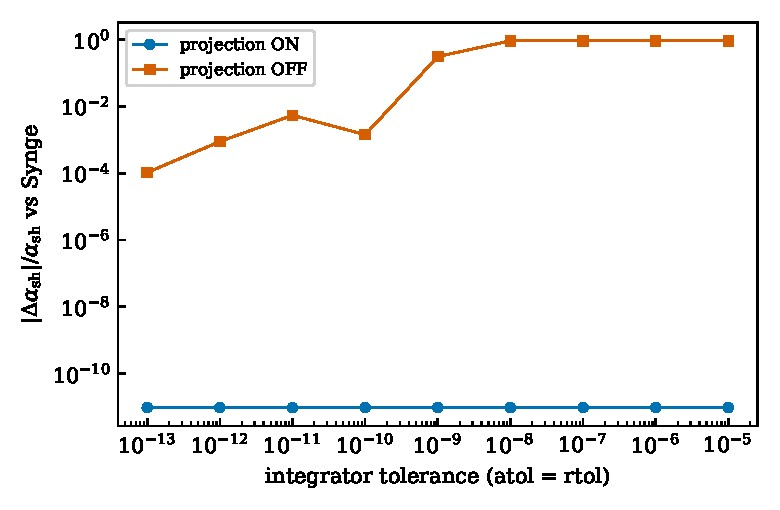
\includegraphics[width=0.72\textwidth]{figures/fig_projection_boundary.pdf}
\caption{The projection experiment: relative deviation of the traced
Schwarzschild shadow angle from the analytic value, versus integrator
tolerance, with the per-step projection \eqref{eq:projection} on and
off. Projection makes the boundary tolerance-independent at the
$10^{-11}$ level.}
\label{fig:projboundary}
\end{figure}

Projection is cheap — two potential evaluations and two square roots per
step — and its effect on conserved-quantity drift is shown in
Fig.~\ref{fig:drifttol}: with projection the reconstructed
$(E, L_z, Q)$ hold to better than $10^{-9}$ along a worst-case grazing
ray at production tolerance, two orders inside the $10^{-6}$ acceptance
gate; without it the drift crosses the gate for all tolerances looser
than $\sim10^{-11}$.

\begin{figure}
\centering
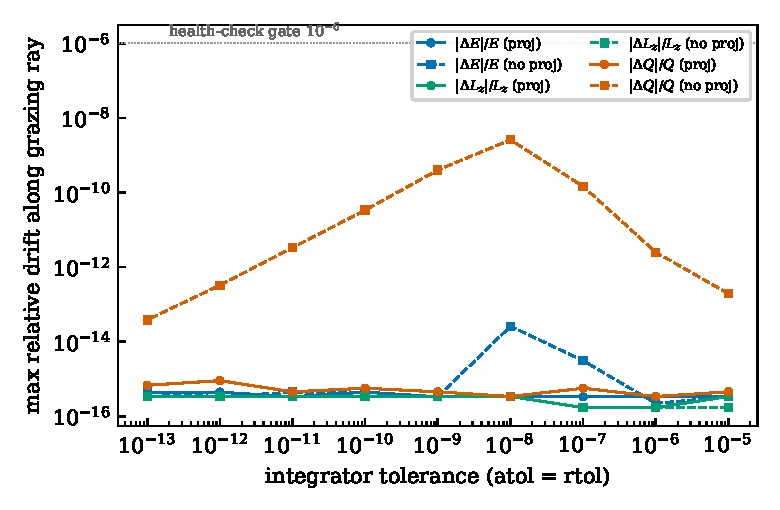
\includegraphics[width=0.8\textwidth]{figures/fig_drift_vs_tol.pdf}
\caption{Maximum relative drift of the reconstructed conserved
quantities along a boundary-grazing ray, versus tolerance, projection on
(circles) and off (squares). The dotted line is the $10^{-6}$
health-check gate enforced by the test suite.}
\label{fig:drifttol}
\end{figure}

A methodological note: projection onto the constraint surface is a
standard tool of geometric integration, but the specific failure it
cures here — long benign propagation amplifying into a classification
error at a distant separatrix — was found empirically, as a
tolerance-dependence of the measured shadow in early Phase-1 runs. The
diagnostic that captured it survives as the hidden \texttt{[.probe]}
test case; the story is told as a methods lesson in
Chapter~\ref{ch:devhistory}.

\section{Complex-step differentiation}
\label{sec:complexstep}

The Hartle--Thorne path (Chapters~\ref{ch:geodesics}, \ref{ch:nohair})
integrates $\mathrm{d}u^\lambda/\mathrm{d}\tau =
-\Gamma^\lambda_{\mu\nu}u^\mu u^\nu$ for arbitrary stationary
axisymmetric metrics, which requires the derivatives
$\partial_r g_{\mu\nu}$, $\partial_\theta g_{\mu\nu}$ of whatever metric
sits behind the \texttt{IMetric} interface. Hand-coding derivatives per
metric invites exactly the class of sign errors this project's test
suite exists to prevent; finite differences trade a truncation error
($\propto h^2$) against a cancellation error ($\propto
\varepsilon_{\rm mach}/h$), bottoming out near $10^{-10}$ relative at
best.

The \emph{complex-step} method \citep{SquireTrapp1998} evades the
trade-off entirely. For a real-analytic $f$, Taylor expansion along the
imaginary axis gives
\begin{equation}
f(x + ih) = f(x) + ih f'(x) - \frac{h^2}{2}f''(x)
- i\frac{h^3}{6}f'''(x) + \cdots
\end{equation}
so that
\begin{equation}
f'(x) = \frac{\operatorname{Im} f(x + ih)}{h} + \mathcal{O}(h^2),
\label{eq:cstep}
\end{equation}
with \emph{no subtraction of nearby quantities anywhere}: the imaginary
part is extracted, not differenced, so $h$ may be made absurdly small.
The implementation uses $h = 10^{-100}$
(\texttt{christoffel} in \texttt{metric.cpp}); the $\mathcal{O}(h^2)$
truncation term is $10^{-200}$, far below the $10^{-308}$ double
underflow only when multiplied by the third derivative — in practice the
result is $f'$ to full machine precision, verified against the
hand-derived Kerr Christoffels in the unit tests. The only requirement
is that the metric components be evaluable on complex arguments, which
is why \texttt{kerr\_components} and the Hartle--Thorne functions are
templated on the scalar type and every \texttt{IMetric} exposes a
\texttt{std::complex<double>} overload.

\section{Convergence behaviour}
\label{sec:convergence}

Fig.~\ref{fig:drifttol} doubles as the convergence study: with
projection off, the conserved-quantity drift scales essentially linearly
with the requested tolerance across eight decades — the signature of a
correctly implemented error estimate (the controller holds the
\emph{local} error at tolerance; the accumulated drift inherits it) —
while with projection on, the drift saturates at the projection floor
($10^{-9}$--$10^{-12}$, set by the guard band near turning points)
independent of tolerance. Both behaviours are the expected ones; their
intersection fixes the production tolerance ($10^{-11}$) as the point
beyond which tightening buys nothing measurable. The
timelike path is validated independently: the rosette integration of
Fig.~\ref{fig:rosettefig} holds $|g_{\mu\nu}u^\mu u^\nu + 1| \lesssim
10^{-13}$ over six radial periods, and the S2 production orbits carry
the same diagnostic through every fit iteration
(Chapter~\ref{ch:devhistory}).
